As PyGrace is still young, the only method yet available to install it
is to download the source code from:

\begin{command}
http://sourceforge.net/projects/pygrace
\end{command}

\noindent
The subsection titled \textit{Installing a development version}
describes how to download the source code.

\subsection*{Installing a development version}

\begin{flushleft}

To check out the PyGrace repository, change to a directory where you
want to put PyGrace, and type:

\begin{command}
svn co https://pygrace.svn.sourceforge.net/svnroot/pygrace/trunk
PyGrace
\end{command}

\begin{figure}[t!]
  \centering
  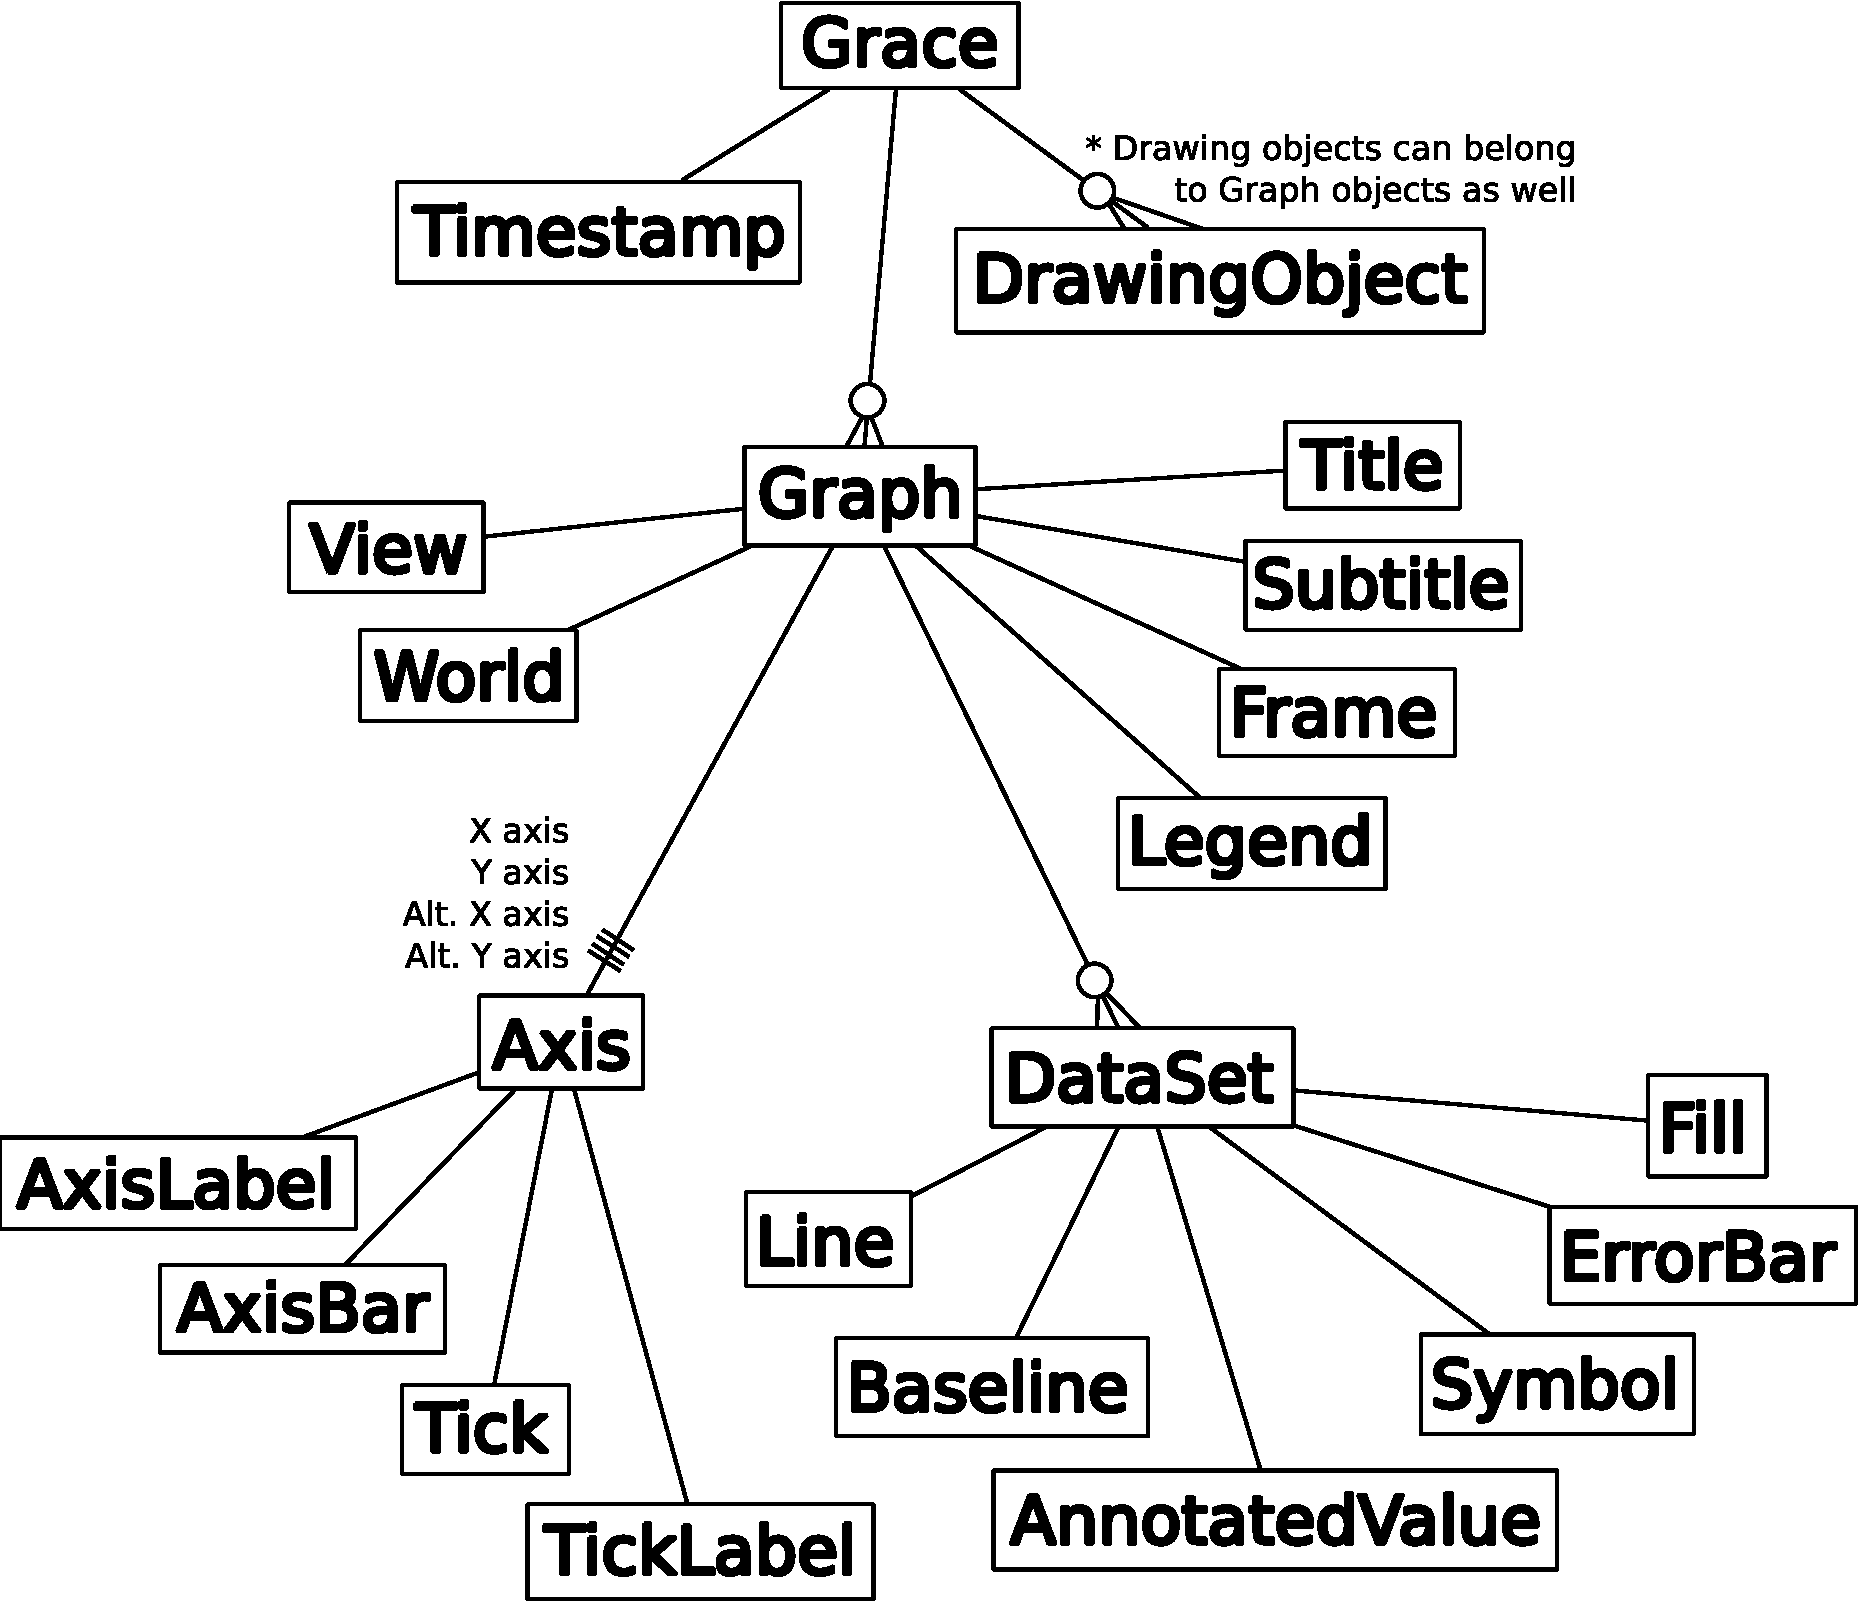
\includegraphics[width=0.67\textwidth]{crow_diagram.pdf}
  \caption{
%
The inheritance structure of PyGrace mirrors the file structure of
Grace.  This diagram uses ``crow's foot'' notation to indicate the
relationship between different entities.
%
  }
  \label{crowdiagram}
\end{figure}

For now, it is important to use the ``correct'' capitalization of
PyGrace (capital P and G).  Then, make sure that the directory you are
in is on the python path (the {\tt PYTHONPATH} environment variable).
One convenient way to do this is to add a line in your
{\tt \textasciitilde/.bashrc} file that says:

\begin{command}
export PYTHONPATH:\$PYTHONPATH:/path/to/your/pybrary/
\end{command}

Notice that, unlike the lame-ass author of this documentation, it is
not necessary to call the directory that PyGrace is located ``the
pybrary.''  After the location of PyGrace is on the {\tt PYTHONPATH},
import statement in python scripts will look in that directory
({\tt \dots/pybrary/}) for modules, and since PyGrace is a package (it
has an {\tt \_\_init\_\_.py} file in the directory), the directory act
like a module.  Now, make sure that you have executed the
{\tt \textasciitilde/.bashrc} file by running

\begin{command}
source \textasciitilde/.bashrc
\end{command}

That should do the trick.  You can test that python can find the
PyGrace package by opening an interactive python prompt and typing

\begin{command}
import PyGrace
\end{command}

If no error is raised, then installation was succesful!

\end{flushleft}


